\documentclass[../Head/Main.tex]{subfiles}
\begin{document}
	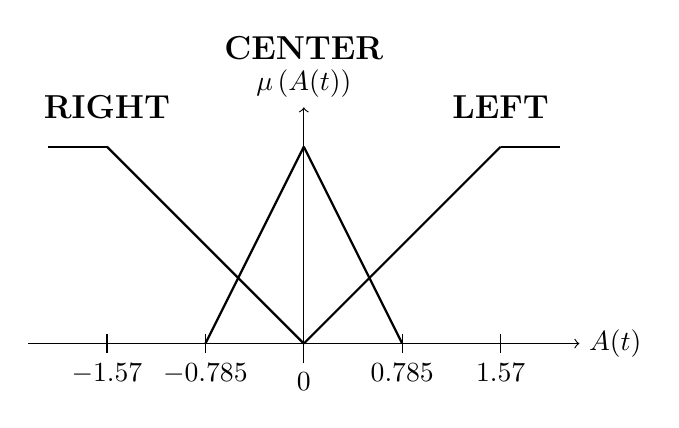
\begin{tikzpicture}
		\draw [->](3,-0.25)--(3,3) node[anchor = south]{$\mu\left(A(t)\right)$};
		\draw [->](-0.5,0)--(6.5,0) node[right]{$A(t)$};
		\node[anchor = north] at (3,-0.25) {$0$};
		
		\node at (0.5,3) {\large\bfseries RIGHT};
		\node at (5.5,3) {\large\bfseries LEFT};
		\node at (3,3.75) {\large\bfseries CENTER};	
		
		\draw (0.5,0.125) -- (0.5,-0.125) 
			node[anchor = north] {$-1.57$};
			
		\draw (5.5,0.125) -- (5.5,-0.125)
			node[anchor = north] {$1.57$};
		
		\draw (1.75,0.125) -- (1.75,-0.125)
			node[anchor = north] {$-0.785$};
			
		\draw (4.25,0.125) -- (4.25,-0.125)
			node[anchor = north] {$0.785$};	
		
		\draw[thick] (-0.25,2.5) -- (0.5,2.5);
		\draw[thick] (5.5,2.5) -- (6.25,2.5);
		
		\draw[thick] (0.5,2.5) -- (3,0);
		\draw[thick] (5.5,2.5) -- (3,0);
		
		\draw[thick] (1.75,0) -- (3,2.5);
		\draw[thick] (4.25,0) -- (3,2.5);
		
		%\node at (2.65,3) {$h$};
		%\node[right] at (3.17, 2.8) {$c$};
		%\node at (3.4,3.4) {$\theta$};
		
	\end{tikzpicture}
\end{document}